%%%%%%%%%%%%%%%%%%%%%%%%
% Compile with XeLaTeX %
%%%%%%%%%%%%%%%%%%%%%%%%

\documentclass{beamer}\usepackage[]{graphicx}\usepackage[]{color}
% maxwidth is the original width if it is less than linewidth
% otherwise use linewidth (to make sure the graphics do not exceed the margin)
\makeatletter
\def\maxwidth{ %
  \ifdim\Gin@nat@width>\linewidth
    \linewidth
  \else
    \Gin@nat@width
  \fi
}
\makeatother

\definecolor{fgcolor}{rgb}{0.345, 0.345, 0.345}
\makeatletter
\@ifundefined{AddToHook}{}{\AddToHook{package/xcolor/after}{\definecolor{fgcolor}{rgb}{0.345, 0.345, 0.345}}}
\makeatother
\newcommand{\hlnum}[1]{\textcolor[rgb]{0.686,0.059,0.569}{#1}}%
\newcommand{\hlstr}[1]{\textcolor[rgb]{0.192,0.494,0.8}{#1}}%
\newcommand{\hlcom}[1]{\textcolor[rgb]{0.678,0.584,0.686}{\textit{#1}}}%
\newcommand{\hlopt}[1]{\textcolor[rgb]{0,0,0}{#1}}%
\newcommand{\hlstd}[1]{\textcolor[rgb]{0.345,0.345,0.345}{#1}}%
\newcommand{\hlkwa}[1]{\textcolor[rgb]{0.161,0.373,0.58}{\textbf{#1}}}%
\newcommand{\hlkwb}[1]{\textcolor[rgb]{0.69,0.353,0.396}{#1}}%
\newcommand{\hlkwc}[1]{\textcolor[rgb]{0.333,0.667,0.333}{#1}}%
\newcommand{\hlkwd}[1]{\textcolor[rgb]{0.737,0.353,0.396}{\textbf{#1}}}%
\let\hlipl\hlkwb

\usepackage{framed}
\makeatletter
\newenvironment{kframe}{%
 \def\at@end@of@kframe{}%
 \ifinner\ifhmode%
  \def\at@end@of@kframe{\end{minipage}}%
  \begin{minipage}{\columnwidth}%
 \fi\fi%
 \def\FrameCommand##1{\hskip\@totalleftmargin \hskip-\fboxsep
 \colorbox{shadecolor}{##1}\hskip-\fboxsep
     % There is no \\@totalrightmargin, so:
     \hskip-\linewidth \hskip-\@totalleftmargin \hskip\columnwidth}%
 \MakeFramed {\advance\hsize-\width
   \@totalleftmargin\z@ \linewidth\hsize
   \@setminipage}}%
 {\par\unskip\endMakeFramed%
 \at@end@of@kframe}
\makeatother

\definecolor{shadecolor}{rgb}{.97, .97, .97}
\definecolor{messagecolor}{rgb}{0, 0, 0}
\definecolor{warningcolor}{rgb}{1, 0, 1}
\definecolor{errorcolor}{rgb}{1, 0, 0}
\makeatletter
\@ifundefined{AddToHook}{}{\AddToHook{package/xcolor/after}{
\definecolor{shadecolor}{rgb}{.97, .97, .97}
\definecolor{messagecolor}{rgb}{0, 0, 0}
\definecolor{warningcolor}{rgb}{1, 0, 1}
\definecolor{errorcolor}{rgb}{1, 0, 0}
}}
\makeatother
\newenvironment{knitrout}{}{} % an empty environment to be redefined in TeX

\usepackage{alltt}

  % Beamer settings
  % \usetheme{Berkeley}
  \usetheme{CambridgeUS}
  % \usecolortheme{dove}
  % \usecolortheme{rose}
  \usecolortheme{seagull}
  \usefonttheme{professionalfonts}
  \usefonttheme{serif}
  \setbeamertemplate{bibliography item}{}

  % Packages and settings
  \usepackage{fontspec}
    \setmainfont{Charis SIL}
  \usepackage[style=apa, backend=biber]{biblatex}
    \addbibresource{References.bib}
  \usepackage{hyperref}
    \hypersetup{colorlinks=true, allcolors=blue}
  \usepackage{siunitx}
    \sisetup{group-minimum-digits=4,
             group-separator={,},
             detect-all}
  \usepackage{graphicx}
    \graphicspath{{./figure/}}
  \usepackage[normalem]{ulem}

  % Document information
  \title[Ethnicity and subject pronouns]{Dissertation Proposal: The relationship between ethnicity and subject pronouns in Louisiana French}
  \author{Joshua McNeill}
  \institute{University of Georgia}
  \date{6 July 2022}

  % New commands
  \newcommand{\orth}[1]{$\langle$#1$\rangle$}
  \newcommand{\lexi}[1]{\textit{#1}}
  \newcommand{\gloss}[1]{`#1'}
\IfFileExists{upquote.sty}{\usepackage{upquote}}{}
\begin{document}
  % <<settings_load_scripts, echo = FALSE>>=
  % read_chunk("analysis.R")
  % opts_chunk$set(echo = FALSE,
  %                warning = FALSE,
  %                message = FALSE,
  %                results = "asis")
  % @
  % <<load_packages_functions_data>>=
  % @
  \begin{frame}
    \titlepage
    \tiny{
      Data and code available at \url{https://osf.io/sy7uq/}.
    }
  \end{frame}

  \begin{frame}
    \tableofcontents[hideallsubsections]
  \end{frame}

  \AtBeginSection[]{
    \begin{frame}
      \tableofcontents[currentsection,
                       hideallsubsections]
    \end{frame}
  }

  \section{Ethnicity in South Louisiana}
    \begin{frame}{South Louisiana}
      \begin{center}
        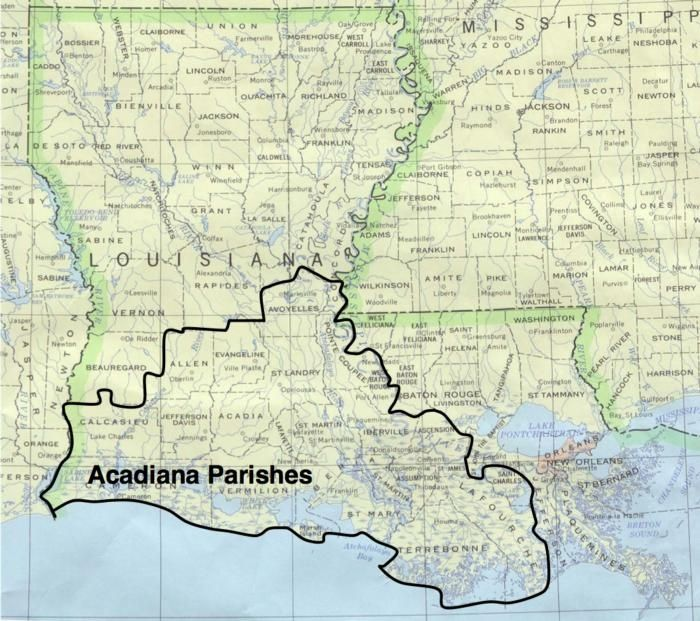
\includegraphics[scale=0.27]{acadiana.jpg}
      \end{center}
      A good place to explore fractal recursivity \parencite{irvine_language_2000}
    \end{frame}

    \begin{frame}{Major Ethnic Groups}
      \begin{center}
        \begin{tabular}{l | l | l}
          Era          & Creoles                                          & Cajuns \\
          \hline
                       &                                                  & \\
          18th century & \parbox[t]{3cm}{Europeans born in the New World} & \parbox[t]{3cm}{Descendents of Acadians} \\
                       &                                                  & \\
          19th century & \parbox[t]{3cm}{Free people of color}            & -- \\
                       &                                                  & \\
          20th century & \parbox[t]{3cm}{Black South Louisianians}        & \parbox[t]{3cm}{White South Louisianians} \\
                       &                                                  & \\
          \hline
        \end{tabular}
      \end{center}
      \begin{center}
        French is still spoken by both groups
      \end{center}
      {\tiny
        \begin{itemize}
          \item Creole sources: \textcite{fortier_french_1884, susberry_racial_2004, neumann_creole_1985}
          \item Cajun sources: \textcite{brown_pronominal_1988, johnson_louisiana_1976, neumann_creole_1985, smith_influence_1939, giancarlo_dont_2019}
        \end{itemize}
      }
    \end{frame}

  \section{Louisiana French}
    \begin{frame}{Subject Pronouns}
      \begin{center}
        {\footnotesize
        \begin{tabular}{l l l}
                    &                                          & \\
          Variable  & Description                              & Variants \\
          \hline
          (1sg)     & 1st person singular                      & \lexi{je}, \lexi{mo}, ø \\
          (2sg.T)   & 2nd person singular T form               & \lexi{tu}, \lexi{to} \\
          (2sg.V)   & 2nd person singular V form               & \lexi{vous}, \lexi{tu}, \lexi{to} \\
          (imp)     & Impersonal pronoun                       & \lexi{on}, \lexi{tu}, \lexi{vous}, \lexi{to} \\
          (3sg.AF)  & 3rd person singular animate feminine     & \lexi{elle}, \lexi{li} \\
          (3sg.AM)  & 3rd person singular animate masculine    & \lexi{il}, \lexi{li} \\
          \textcolor{orange}{(3sg.IF)}  & 3rd person singular inanimate feminine   & \lexi{ça}, \lexi{elle}, \lexi{li} \\
          \textcolor{orange}{(3sg.IM)}  & 3rd person singular inanimate masculline & \lexi{ça}, \lexi{il}, \lexi{li} \\
          (expl)    & Expletive pronoun                        & \lexi{il}, \lexi{ça} \\
          (1pl)     & 1st person plural                        & \lexi{nous}, \lexi{nous-autres}, \lexi{on} \\
          (2pl)     & 2nd person plural                        & \lexi{vous}, \lexi{vous-autres}, \lexi{zo}, \lexi{tu} \\
          \textcolor{purple}{(3pl.F)}   & 3rd person plural feminine               & \lexi{elles}, \lexi{ça}, \lexi{eux}, \lexi{eux-autres}, \lexi{yé} \\
          \textcolor{purple}{(3pl.M)}   & 3rd person plural masculine              & \lexi{ils}, \lexi{ça}, \lexi{eux}, \lexi{eux-autres}, \lexi{yé} \\
        \end{tabular}
        }
      \end{center}
    \end{frame}

    \begin{frame}{Previous Research}
      \begin{itemize}
        \item (3pl) differed between Cajuns and Houma Indians \parencite{rottet_language_1995, dajko_ethnic_2009}
        \begin{itemize}
          \item Other pronouns were examined but not significant for ethnicity
        \end{itemize}
        \item (1sg) has been examined but not for ethnic variation \parencite{carmichael_language_2019, gudmestad_variationist_2022, klingler_probleme_2005}
        \begin{itemize}
          \item As has (3pl) but, again, not for ethnic variation \parencite{byers_defining_1988, klingler_if_2003, neumann_creole_1985}
        \end{itemize}
        \item Subject pronouns have been examined in other varieties in numerous ways \parencite{lambert_use_1967, schoch_probleme_1978}
      \end{itemize}
    \end{frame}

    \begin{frame}{Research Questions}
      \begin{itemize}
        \item[RQ1:] Do subject pronouns vary in Louisiana French between Cajun and Creole speakers, and what role does race play in this variation?
        \item[RQ2:] How does the homophily or lack thereof in the ethnic make-up of personal networks among French speakers in South Louisiana relate to variation in subject pronoun usage?
        \item[RQ3:] What do Louisiana French speakers participating in this study have to say about ethnicity and race?
      \end{itemize}
    \end{frame}

  \section{Methods}
    \begin{frame}{Sample}
      \begin{itemize}
        \item Snowball sampling \parencite{brown_pronominal_1988, giancarlo_dont_2019, rottet_language_1995}
        \item 30 participants $\times$ 1 hour each $\to$ 1,750 tokens per variable on average
        \item Participants identify as Creole or Cajun
      \end{itemize}
      \begin{center}
        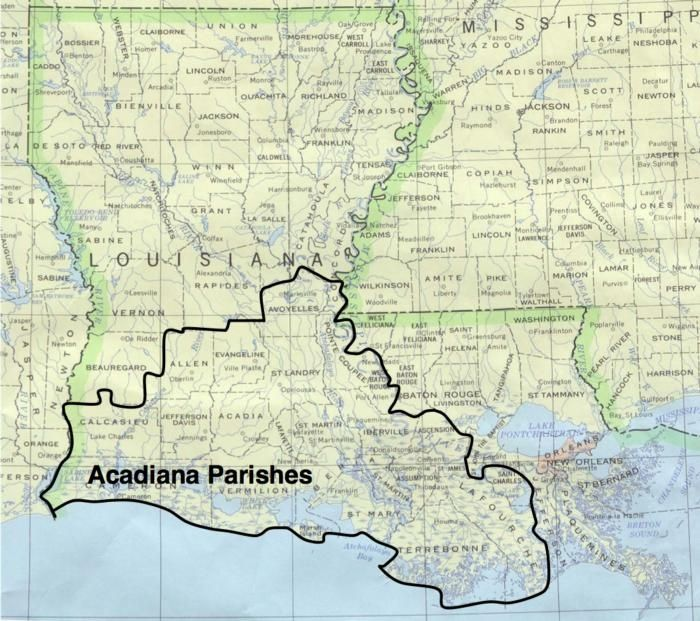
\includegraphics[scale=0.2]{acadiana.jpg}
      \end{center}
    \end{frame}

    \begin{frame}{Social Variables}
      \centering
      \begin{tabular}{l l}
                          & \\
        Social Variable   & Levels \\
        \hline
        \emph{Ethnicity}  & Creole, Cajun \\
        French Background & naturalistic, institutional, personal \\
        Gender            & man, woman, other answer \\
        Birth Year        & continuous numeric \\
        Residence         & parish \\
        Raised            & parish \\
        Profession        & blue and white collar \\
        Education         & \parbox[t]{6cm}{some school, high school graduate, college graduate} \\
        Race              & \parbox[t]{6cm}{singular White, singular Black, border, protean, transcendent \parencite{rockquemore_beyond_2007}}
      \end{tabular}
    \end{frame}

    \begin{frame}{RQ1 Analysis}
      \begin{itemize}
        \item[RQ1:] Do subject pronouns vary in Louisiana French between Cajun and Creole speakers, and what role does race play in this variation?
      \end{itemize}
      \vspace{0.5cm}
      \begin{equation*}
        \begin{aligned}
          \text{Pronoun}\  & \~{}\  \text{Social Variables}\  +\\
                           & \text{Verb.Type}\  +\\
                           & \text{Network.Ethnic.Homophily}\  +\\
                           & (1|\text{Participant})\  +\  (1|\text{Following.Verb})
        \end{aligned}
      \end{equation*}
      \begin{itemize}
        \item Binomial or multinomial logistic models based on the levels of the pronoun
        \item Variance inflation factor (VIF) for auto-correlated factors
        \item Akaike information criterion (AIC) for model selection
      \end{itemize}
    \end{frame}

    \begin{frame}{RQ2 Analysis}
      \begin{itemize}
        \item[RQ2:] How does the homophily or lack thereof in the ethnic make-up of personal networks among French speakers in South Louisiana relate to variation in subject pronoun usage?
      \end{itemize}
      \vspace{0.5cm}
      \begin{equation*}
        \text{French.Frequency}\  \~{}\  \text{Alter.Type}\  +\  (1|\text{Participant})
      \end{equation*}
      \vspace{0.5cm}
      \begin{tabular}{l l l l}
        Stat                                        & Stat                                            & Test            & $N$ \\
        \hline
        \parbox[t]{4cm}{Mean ethnic homophily\\of francophone alters} & \parbox[t]{4cm}{Mean ethnic homophily\\of non-francophone alters} & Paired $t$-test & 60 \\
        \hline
        \parbox[t]{4cm}{Mean ethnic homophily\\for Creoles}           & \parbox[t]{4cm}{Mean ethnic homophily\\for Cajuns}             & $t$-test        & 30 \\
      \end{tabular}
    \end{frame}

  \section{Impact}
    \begin{frame}{}
      \begin{itemize}
        \item Better understanding fractal recursivity
        \item Better understanding the role of race in the general US on understanding of local social categories
        \item Add to the descriptive literature on heritage languages
      \end{itemize}
    \end{frame}

  \section{References}
    \printbibliography

    \begin{frame}{}
      \begin{center}
        Questions and comments?
      \end{center}
    \end{frame}

    \begin{frame}{General Characteristics}
      \begin{itemize}
        \item Explicit progressive aspect expressed with \lexi{après} \parencite{papen_structural_1997}
        \item /ʒ/ produced as [h] \parencite{carmichael_language_2019}
        \begin{itemize}
          \item \lexi{[h]'ai [h]amais man[h]é ça.}
          \item \gloss{I've never eaten that.}
        \end{itemize}
        \item {}[ɾ] where most varieties have [ʀ] or [ʁ] \parencite{blainey_first_2013}
        \begin{itemize}
          \item \lexi{ap[ɾ]ès} \gloss{after}
          \item \lexi{[ɾ]aison} \gloss{reason}
        \end{itemize}
      \end{itemize}
    \end{frame}

    \begin{frame}{Likely Collapsed Variables}
      \centering
      \begin{tabular}{c c}
        (3g.IF)                                                                  & (3g.IM) \\
        \lexi{ça}, \sout{\lexi{elle}}, \lexi{li}                                 & \lexi{ça}, \sout{\lexi{il}}, \lexi{li} \\
                                                                                 & \\
        \multicolumn{2}{c}{(3g.I)} \\
        \multicolumn{2}{c}{\lexi{ça}, \lexi{li}} \\
                                                                                 & \\
        \hline
                                                                                 & \\
        (3pl.F)                                                                  & (3pl.M) \\
        \sout{\lexi{elles}}, \lexi{ça}, \lexi{eux}, \lexi{eux-autres}, \lexi{yé} & \lexi{ils}, \lexi{ça}, \lexi{eux}, \lexi{eux-autres}, \lexi{yé} \\
                                                                                 & \\
        \multicolumn{2}{c}{(3pl)} \\
        \multicolumn{2}{c}{\lexi{ils}, \lexi{ça}, \lexi{eux}, \lexi{eux-autres}, \lexi{yé}} \\
      \end{tabular}
    \end{frame}
\end{document}
